\section{Algoritmos para lenguajes libres de contexto}
\subsection{Autómatas apiladores}
\subsubsection{Versión normal}

\fig{img/cap5/idea_automata.png}{0.7}{Idea de un autómata apilador}

\paragraph*{Definición.} Un autómata apilador (\textit{PushDown Automata}, PDA) es una estructura:
\alignformula{
    \ca{P}=(Q,\Sigma,\Gamma,\Delta,q_0,\bot,F)
}
\begin{itemize}
    \item $Q$ es un conjunto finito de \textbf{estados}.
    \item $\Sigma$ es el alfabeto del \textbf{input}.
    \item $q_0 \in Q$ es el estado \textbf{inicial}.
    \item $F$ es el conjunto de estados \textbf{finales}.
    \item $\Gamma$ es el alfabeto de \textbf{stack}.
    \item $\bot \in \Gamma$ es el símbolo \textbf{inicial del stack} (fondo).
    \item $\Delta \subseteq(Q \times(\Sigma \cup\{\epsilon\}) \times \Gamma) \times\left(Q \times \Gamma^*\right)$ es una relación finita de transición.
\end{itemize}

Intuitivamente, la transición:
\alignformula{
    \Big((p,a,A),(q,B_1B_2\cdots B_k)\Big) \in \Delta
}
si el autómata apilador está:
\begin{itemize}
    \item en el estado $p$, leyendo $a$, y en el tope del stack hay una $A$,
\end{itemize}
entonces:
\begin{itemize}
    \item cambia al estado $q$, y modifico el tope $A$ por $B_1B_2\cdots B_k$.
\end{itemize}

Intuitivamente, la transición \textbf{en vacío}:
\alignformula{
    \Big((p,\epsilon,A),(q,B_1B_2\cdots B_k)\Big) \in \Delta
}
si el autómata apilador está:
\begin{itemize}
    \item en el estado $p$, \textit{sin lectura de una letra}, y en el tope del stack hay una $A$,
\end{itemize}
entonces:
\begin{itemize}
    \item cambia al estado $q$, y modifico el tope $A$ por $B_1B_2\cdots B_k$.
\end{itemize}

\ejemplo{}{}{
    $$
        \ca{P}=(Q,\Sigma,\Gamma,\Delta,q_0,\bot,\{q_f\})
    $$
    \begin{itemize}
        \item $Q=\{q_0,q_1,q_f\}$, $\Sigma = \{a,b\}$, $\Gamma = \{A,\bot\}$ y $\Delta$:
              $$
                  \begin{array}{ll}
                      \left(q_0, a, \perp, q_0, A \perp\right)         & q_0 \perp \stackrel{a}{\rightarrow} q_0 A \perp \\
                      \left(q_0, a, A, q_0, A A\right)                 & q_0 A \stackrel{a}{\rightarrow} q_0 A A         \\
                      \left(q_0, b, A, q_1, \epsilon\right)            & q_0 A \stackrel{b}{\rightarrow} q_1             \\
                      \left(q_1, b, A, q_1, \epsilon\right)            & q_1 A \stackrel{b}{\rightarrow} q_1             \\
                      \left(q_1, \epsilon, \perp, q_f, \epsilon\right) & q_1 \perp \stackrel{\epsilon}{\rightarrow} q_f
                  \end{array}
              $$
    \end{itemize}

    \img{img/cap5/ejemplo1.png}{0.65}
}

\paragraph*{Notación.} Dada una palabra $A_1A_2\ldots A_k \in \Gamma^+$ decimos que:
\begin{itemize}
    \item $A_1 A_2 \ldots A_k$ es un stack (contenido),
    \item $A_1$ es el \textbf{tope} del stack y
    \item $A_2 \ldots A_k$ es la \textbf{cola} del stack.
\end{itemize}

\paragraph*{Definición.} Una \textbf{configuración} de $\ca{P}$ es una tupla $(q\cdot \gamma, w) \in (Q\cdot \Gamma^*, \Sigma^*)$ tal que:
\begin{itemize}
    \item $q$ es el estado actual.
    \item $\gamma$ es el contenido del stack.
    \item $w$ es el contenido del input.
\end{itemize}
Decimos que una configuración:
\alignformula{
    (q\cdot \gamma, w) \in (Q\cdot \Gamma^*, \Sigma^*)
}
\begin{itemize}
    \item es \textbf{inicial} si $q\cdot \gamma = q_0\cdot \bot$.
    \item es \textbf{final} si $q\cdot \gamma = q_f\cdot \epsilon$ con $q_f \in F$ y $w=\epsilon$.
\end{itemize}

\paragraph*{Definición.} Se define la relación $\vdash_{\ca{P}}$ de \textbf{siguiente-paso} entre configuraciones de $\ca{P}$:
\alignformula{
    \left(q_1 \cdot \gamma_1, w_1\right) \quad \vdash_{\mathcal{P}} \quad\left(q_2 \cdot \gamma_2, w_2\right)
}
si, y sólo si, existe una transición $\left(q_1, a, A, q_2, \alpha\right) \in \Delta \text { y } \gamma \in \Gamma^*$ tal que:
\begin{itemize}
    \item $w_1 = a \cdot w_2$
    \item $\gamma_1 = A\cdot \gamma$
    \item $\gamma_2 = \alpha \cdot \gamma$
\end{itemize}

Se define $\vdash_{\ca{P}}^*$ como la clausura \textbf{refleja} y \textbf{transitiva} de $\vdash_\ca{P}$. En otras palabras:
\alignformula{
    \begin{gathered}
        \left(q_1 \gamma_1, w_1\right) \vdash_{\mathcal{P}}^*\left(q_2 \gamma_2, w_2\right) \text { si uno puede ir de }\left(q_1 \gamma_1, w_1\right) \text { a }\left(q_2 \gamma_2, w_2\right) \\
        \text { en } 0 \text { o más pasos. }
    \end{gathered}
}
\ejemplo{}{}{
    Para la palabra $w=aaabbb$, tenemos la ejecución:
    \img{img/cap5/ejemplo2.png}{0.7}
}

\paragraph*{Definiciones.} $\cal{P}$ \textbf{acepta} $w$ si, y sólo si, $\left(q_0 \perp, w\right) \vdash_{\mathcal{P}}^*\left(q_f, \epsilon\right)$ para algún $q_f \in F$.

\hspace{70pt} El \textbf{lenguaje aceptado} por $\ca{P}$ se define como:
\alignformula{
    \ca{L}(\ca{P})=\{w\in \Sigma^*\| \ \ca{P} \text{ acepta } w\}
}
\ejemplo{}{}{
    El lenguaje aceptado por el PDA utilizado en los ejemplos anteriores es $\ca{L}(\ca{P})=\{a^nb^n\ | \ n \ge 0\}$.
}

\subsubsection{Versión alternativa}
Esta definición de autómata apilador es poco común pero trae algunas ventajas:
\begin{itemize}
    \item Es un modelo que ayuda a entender mejor los algoritmos de evaluación para gramáticas.
    \item Es un modelo menos estándar pero mucho más sencillo.
    \item Al profe Cristian le gustó y lo encontró interesante.
\end{itemize}

\paragraph*{Definición.} Un \textbf{PDA alternativo} es una estructura:
\alignformula{
    \ca{D}=(Q,\Sigma,\Delta,q_0,F)
}
\begin{itemize}
    \item $Q$ es un conjunto finito de \textbf{estados}.
    \item $\Sigma$ es el alfabeto del \textbf{input}.
    \item $q_0 \in Q$ es el estado \textbf{inicial}.
    \item $F$ es el conjunto de estados \textbf{finales}.
    \item $\Delta \subseteq Q^+ \times (\Sigma \cup \{\epsilon\})\times Q^*$ es una \textbf{relación finita de transición}.
\end{itemize}
Intuitivamente, la transición:
\alignformula{
    \Big( A_1\ldots A_i, a, B_1 \ldots B_j \Big) \in \Delta
}
si el autómata apilador tiene:
\begin{itemize}
    \item $A_1\ldots A_i$ en el tope del stack y leyendo $a$,
\end{itemize}
entonces:
\begin{itemize}
    \item cambia el tope $A_1\ldots A_i$ por $B_1\ldots B_j$.
\end{itemize}

En este tipo de autómata apilador, \textbf{no hay diferencia} entre estados y alfabeto del stack.

\paragraph*{Definición.} Una \textbf{configuración} de $\ca{D}$ es una tupla
\alignformula{
    (q_1\ldots q_k, w) \in (Q^+,\Sigma^*)
}
tal que:
\begin{itemize}
    \item $q_1\ldots q_k$ es el contenido del stack con $q_1$ el tope del stack.
    \item $w$ es el contenido del input.
\end{itemize}
Decimos que una configuración:
\begin{itemize}
    \item $(q_0,w)$ es \textbf{inicial}.
    \item $(Q_f,\epsilon)$ es \textbf{final} si $q_f \in F$.
\end{itemize}

\paragraph*{Definición.} Se define la relación $\vdash_{\ca{D}}$ de \textbf{siguiente-paso} entre configuraciones de $\ca{D}$:
\alignformula{
    \left( \gamma_1, w_1\right) \quad \vdash_{\mathcal{D}} \quad\left(\gamma_2, w_2\right)
}
si, y sólo si, existe una transición $\left(\alpha, a, \beta\right) \in \Delta \text { y } \gamma \in \Gamma^*$ tal que:
\begin{itemize}
    \item $w_1 = a \cdot w_2$
    \item $\gamma_1 = \alpha\cdot \gamma$
    \item $\gamma_2 = \beta \cdot \gamma$
\end{itemize}

Se define $\vdash_{\ca{D}}^*$ como la clausura \textbf{refleja} y \textbf{transitiva} de $\vdash_\ca{D}$.

\paragraph*{Definiciones.} $\ca{D}$ \textbf{acepta} $w$ si, y sólo si, $(q_0,w) \vdash_\ca{D}^* (q_f,\epsilon)$ para algún $q_f \in F$. Además, el \textbf{lenguaje aceptado} por $\ca{D}$ se define como:
\alignformula{
    \ca{L}(\ca{D})=\{w\in \Sigma^*\| \ \ca{D} \text{ acepta } w\}
}

\newpage
\ejemplo{}{}{
    $$
        \ca{D}=(Q,\{a,b\},\Delta,q_0,F)
    $$
    \begin{itemize}
        \item $Q=\{\bot, q_0, q_1, q_f\}$ y $\Delta$:
              \img{img/cap5/ejemplo4.png}{0.6}
    \end{itemize}
    $$
        \ca{L}(\ca{D})=\{a^nb^n \ |\ n\ge 1\}
    $$
}

\teorema{}{}{
    Para todo autómata apilador $\ca{P}$ existe un autómata apilador alternativo $\ca{D}$, y viceversa, tal que:
    $$
        \ca{L}(\ca{P}) = \ca{L}(\ca{D})
    $$
}
El teorema anterior nos dice que podemos usar ambos modelos de manera \textbf{equivalente}.

\subsectionmark{PDA versus CFG}
\subsection{Autómatas apiladores vs gramáticas libres de contexto}
\subsectionmark{PDA versus CFG}
¿En qué se parecen CFG a PDA?
\fig{img/cap5/cfg_vs_pda.png}{0.3}{Gramáticas vs Autómatas apiladores}

\teorema{}{}{
    Todo \textbf{lenguaje libre de contexto} puede ser descrito equivalentemente por:
    \begin{itemize}
        \item Una gramática libre de contexto (\textbf{CFG}).
        \item Un autómata apilador (\textbf{PDA}).
    \end{itemize}
}

\subsubsection{Desde CFG a PDA}
Partimos enunciado un teorema:
\teorema{}{}{
    Para toda gramática libre de contexto $\ca{G}$, existe un \textbf{autómata apilador alternativo} $\ca{D}$, tal que:
    $$
        \ca{L}(\ca{G}) = \ca{L}(\ca{D})
    $$
}

\paragraph*{Construcción $\ca{D}$ desde $\ca{G}$.} Sea $\ca{G}=(V,\Sigma,P,S)$ una CFG. Construimos un PDA alternativo $\ca{D}$ que acepta $\ca{L}(\ca{G})$:
\alignformula{
    \ca{D}=\Big( V \cup \Sigma \cup \{q_0,q_f\}, \Sigma, \Delta, q_0, \{q_f\} \Big)
}
La relación de transición $\Delta$ se define como:
\begin{table}[H]
    \centering
    \begin{tabular}{lllll}
        $\Delta$ & $=$ & $\{ (q_0, \epsilon, S \cdot q_f) \}$               & $\cup$ &                     \\
                 &     & $\{ (X,\epsilon,\gamma)\ | \ X\to \gamma \in P \}$ & $\cup$ & \textbf{(Expandir)} \\
                 &     & $\{ (a,a,\epsilon) \ | \ a \in \Sigma \}$          &        & \textbf{(Reducir)}  \\
                 &     &                                                    &        &
    \end{tabular}
\end{table}
\paragraph*{Demostración $\ca{L}(\ca{G}) = \ca{L}(\ca{D})$.} Debemos demostrar dos direcciones: $\ca{L}(\ca{G}) \subseteq \ca{L}(\ca{D})$ y $\ca{L}(\ca{D}) \subseteq \ca{L}(\ca{G})$.

\paragraph*{Demostración $\ca{L}(\ca{G}) \subseteq \ca{L}(\ca{D})$.} Para cada $w \in \ca{L}(\ca{G})$ debemos encontrar una ejecución de aceptación de $\ca{D}$ sobre $w$. ¿Cómo encontramos esta ejecución? La idea es que para cada árbol de derivación $\ca{T}$ de $\ca{G}$ sobre $w$, construimos una ejecución de $\ca{D}$ sobre $w$ que recorre el árbol $\ca{T}$ \textbf{en profundidad} (DFS). Por tanto, debemos usar \textbf{inducción} sobre la altura del árbol $\ca{T}$.

\paragraph*{Hipótesis de inducción.} Para todo árbol de derivación $\ca{T}$ de $\ca{G}$ con \textbf{altura} $h$ tal que:
\begin{itemize}
    \item la raíz de $\ca{T}$ es $X$, y
    \item $\ca{T}$ produce la palabra $w$
\end{itemize}
entonces $(X\cdot\gamma, w) \vdash_\ca{D}^* (\gamma, \epsilon)$ para todo $\gamma \in Q^+$.

\paragraph{Caso base: $h=1$.} Si $\ca{T}$ tiene altura $1$, entonces:
\begin{itemize}
    \item $\ca{T}$ produce la palabra $w=a$ para algún $a\in \Sigma$ y
    \item $\ca{T}$ consiste de un nodo $X$ y un hijo $a$ con $X \to a$.
\end{itemize}
Entonces para todo $\gamma \in Q^+$:
$$
    (X \cdot \gamma, a) \vdash_\mathcal{D} (a \cdot \gamma, a) \vdash_\mathcal{D}(\gamma, \epsilon)
$$
es una ejecución de $\ca{D}$ sobre $a$.

\paragraph*{Caso inductivo: $h=n$.} Suponemos que el árbol de derivación $\ca{T}$ de $\ca{G}$ tiene \textbf{altura} $n$ tal que:
\begin{itemize}
    \item la raíz de $\ca{T}$ es $X$, y
    \item $\ca{T}$ produce la palabra $w$.
\end{itemize}
\textbf{Sin pérdida de generalidad}, suponga que $\ca{T}$ es de la forma:
\img{img/cap5/dem1.png}{0.5}
donde $w = u\cdot v$ y $X\to YZ$. Por HI, se tiene que para todo $\gamma_1, \gamma_2 \in Q^+$:
$$
    \begin{aligned}
        \left(Y \cdot \gamma_1, u\right) & \vdash_{\mathcal{D}}^*\left(\gamma_1, \epsilon\right) \\
        \left(Z \cdot \gamma_2, v\right) & \vdash_{\mathcal{D}}^*\left(\gamma_2, \epsilon\right)
    \end{aligned}
$$
Para $\gamma \in Q^+$ \textbf{construimos} la siguiente ejecución de $\ca{D}$ sobre $w=uv$:
$$
    (X \cdot \gamma, u v) \vdash_{\mathcal{D}}(Y Z \cdot \gamma, u v) \vdash_{\mathcal{D}}^*(Z \cdot \gamma, v) \vdash_{\mathcal{D}}^*(\gamma, \epsilon)
$$
\hfill $\blacksquare$

La demostración de $\ca{L}(\ca{D}) \subseteq \ca{L}(\ca{G})$ se deja como ejercicio propuesto al lector.

% \paragraph*{Demostración $\ca{L}(\ca{D}) \subseteq \ca{L}(\ca{G})$.} Para cada $w \in \ca{L}(\ca{D})$ debemos encontrar un árbol de derivación de $\ca{G}$ para $w$. ¿Cómo encontramos un árbol de derivación para $w$? La idea es que si tenemos una ejecución de $\ca{D}$ sobre $w$ de la forma:
% $$
%     \left(X \cdot q_f, w\right) \vdash_{\mathcal{D}}^*\left(q_f, \epsilon\right)
% $$
% entonces $X \underset{\mathcal{G}}{\stackrel{\star}{\Rightarrow}} w$. Por tanto, podemos usar \textbf{inducción} en la cantidad de pasos de la ejecución.

% \paragraph{Hipótesis de inducción.} Para toda ejecución de $\ca{D}$ sobre $w$ de largo $k$ de la forma:
% $$
%     \left(X \cdot q_f, w\right)=\left(\gamma_0, w_0\right) \vdash_\mathcal{D}\left(\gamma_1, w_1\right) \vdash_\mathcal{D} \cdots \vdash_\mathcal{D}\left(\gamma_k, w_k\right)=\left(q_f, \epsilon\right)
% $$
% entonces $X \underset{\mathcal{G}}{\stackrel{\star}{\Rightarrow}} w$.

\subsubsection{Desde PDA a CFG}
Partimos enunciando el siguiente teorema:
\teorema{}{}{
    Para todo autómata apilador $\ca{P}$, existe una gramática libre de contexto $\ca{G}$ tal que:
    $$
        \ca{L}(\ca{P}) = \ca{L}(\ca{G})
    $$
}
\paragraph{Demostración $\ca{L}(\ca{P}) = \ca{L}(\ca{G})$.} Sea $\ca{P}=(Q,\Sigma,\Gamma,\Delta,q_0,\bot,F)$ un PDA (normal). Los pasos a seguir son:
\begin{enumerate}
    \item Convertir $\ca{P}$ a un PDA $\ca{P}'$ con \textbf{UN solo estado}.
    \item Convertir $\ca{P}'$ a una gramática libre de contexto $\ca{G}$.
\end{enumerate}

\paragraph{Paso 1.} Sea $\ca{P}=(Q,\Sigma,\Gamma,\Delta,q_0,\bot,F)$ un PDA. Podemos analizar:
\begin{itemize}
    \item ¿Por qué NO necesitamos la información de los estados?
    \item ¿Cómo guardamos la información de los estados en el stack?
\end{itemize}

Esto conlleva a la siguiente pregunta: \textit{Si el PDA está en el estado $p$ y en el tope del stack hay una $A$, ¿a cuál estado llegaré al remover $A$ del stack?} \medbreak

La solución a esta pregunta es que podemos \textbf{adivinar} (no-determinismo) el estado que vamos a llegar cuando removamos $A$ del stack. \medbreak

\textbf{Sin pérdida de generalidad}, podemos asumir que
\begin{enumerate}
    \item Todas las transiciones son de la forma:
          $$
              q A \stackrel{c}{\rightarrow} p B_1 B_2 \quad \text{o} \quad q A \stackrel{c}{\rightarrow} p \epsilon
          $$
          con $c \in (\Sigma \cup \{\epsilon\})$.
    \item Existe $q_f \in Q$ tal que si $w \in \ca{L}(\ca{P})$ entonces:
          $$
              \left(q_0 \bot, w\right) \vdash_{\mathcal{D}}^*\left(q_f, \epsilon\right)
          $$
\end{enumerate}
Estos dos puntos nos aseguran  que siempre llegamos al \textbf{mismo estado} $q_f$. Luego, construimos el autómata apilador $\ca{P}'$ con \textbf{un solo estado}:
$$
    \mathcal{P}^{\prime}=\left(\{q\}, \Sigma, \Gamma^{\prime}, \Delta^{\prime},\{q\}, \perp^{\prime},\{q\}\right)
$$
\begin{itemize}
    \item $\Gamma'= Q\times \Gamma \times Q$.

          \textit{``$(p, A, q) \in \Gamma'$ si desde $p$ leyendo $A$ en el tope del stack llegamos a $q$ al hacer pop de $A$''.}

    \item $\bot' = (q_0,\bot, q_f)$.

          \textit{``El autómata parte en $q_0$ y al hacer pop de $\bot$ llegará a $q_f$''.}

    \item Si $p A \stackrel{c}{\rightarrow} p^{\prime} B_1 B_2 \in \Delta$ con $c \in (\Sigma \cup \{\epsilon\})$, entonces \textbf{para todo} $p_1,p_2 \in Q$:
          $$
              q\left(p, A, p_2\right) \stackrel{c}{\rightarrow} q\left(p^{\prime}, B_1, p_1\right)\left(p_1, B_2, p_2\right) \in \Delta^{\prime}
          $$

    \item Si $p A \stackrel{c}{\rightarrow} p^{\prime}\in \Delta$ con $c \in (\Sigma \cup \{\epsilon\})$, entonces:
          $$
              q\left(p, A, p^{\prime}\right) \stackrel{c}{\rightarrow} q \in \Delta^{\prime}
          $$
\end{itemize}

\paragraph{Hipótesis de inducción (en el número de pasos $n$).} Para todo $p,p' \in Q$, $A \in \Gamma$ y $w \in \Sigma^*$ se cumple que:
$$
    (p A, w) \vdash_{\mathcal{P}}^n\left(p^{\prime}, \epsilon\right) \quad \text { si, y solo si, } \quad\left(q\left(p, A, p^{\prime}\right), w\right) \vdash_{\mathcal{P}^{\prime}}^n(q, \epsilon)
$$
donde $\vdash_\ca{P}^n$ es la relación de \textbf{siguiente-paso} de $\ca{P}$ $n$-veces. \medbreak

Si demostramos esta hipótesis, habremos demostrado que $\ca{L}(\ca{P}) = \ca{L}(\ca{P'})$. ¿Por qué?

\paragraph{Caso base: $n=1$.} Para todo $p,p' \in Q$, y $A \in \Gamma$ se cumple que:
$$
    (p A, c) \vdash_\mathcal{P}\left(p^{\prime}, \epsilon\right) \quad \text { si, y solo si, } \quad\left(q\left(p, A, p^{\prime}\right), c\right) \vdash_{\mathcal{P}^{\prime}}(q, \epsilon)
$$
para todo $c \in (\Sigma \cup \{\epsilon\})$.

\paragraph{Caso inductivo.} \textbf{Sin pérdida de generalidad}, suponga que $pA \overset{a}{\to} p_1A_1A_2$ y $w=auv$, entonces

$$
    (p A, \underbrace{a u v}_w) \vdash_{\mathcal{P}}^n\left(p^{\prime}, \epsilon\right) \text { ssi }(p A, a u v) \vdash_{\mathcal{P}}\left(p_1 A_1 A_2, u v\right) \vdash_{\mathcal{P}}^i\left(p_2 A_2, v\right) \vdash_{\mathcal{P}}^j\left(p^{\prime}, \epsilon\right)
$$
\begin{align*}
     & \text{ssi }  \left(p_1 A_1, u\right) \vdash_{\mathcal{P}}^i\left(p_2, \epsilon\right) \text { y } \quad\left(p_2 A_2, v\right) \vdash_{\mathcal{P}}^j\left(p^{\prime}, \epsilon\right)                                  \\
     & \text {ssi }  \left(q\left(p_1, A_1, p_2\right), u\right) \vdash_{\mathcal{P}^{\prime}}^i(q, \epsilon) \text { y } \quad\left(q\left(p_2, A_2, p^{\prime}\right), v\right) \vdash_{\mathcal{P}^{\prime}}^j(q, \epsilon) \\
     & \text {ssi }  \left.\left(q\left(p, A, p^{\prime}\right), auv\right) \vdash_{\mathcal{P}}\left(q\left(p_1, A_1, p_2\right)\left(p_2, A_2, q\right)\right), u v\right) \vdash_{\mathcal{P}}^{i+j}(q, \epsilon)
\end{align*}

\hfill $\blacksquare$

\paragraph{Paso 2.} Sea $\ca{P}=(\{q\},\Sigma,\Gamma,\Delta,q,\bot,\{q\})$ un PDA con \textbf{UN solo estado}. Construimos la gramática:
$$
    \ca{G} = (V, \Sigma, P, \bot)
$$
\begin{itemize}
    \item $V=\Gamma$.
    \item Si $qA \overset{\epsilon}{\to} q\alpha \in \Delta$ entonces $A \to \alpha \in P$
    \item Si $qA \overset{a}{\to} q\alpha \in \Delta$ entonces $A \to a\alpha \in P$
\end{itemize}
La demostración de este paso queda como ejercicio propuesto al lector.

\subsection{Parsing: cómputo de First y Follow}

\paragraph{Recordatorio.} La \textbf{sintaxis} de un lenguaje es un conjunto de reglas que describen los programas válidos que tienen significado. Por otro lado, la \textbf{semántica} de un lenguaje define el significado de un programa correcto según la sintaxis.
\fig{img/cap5/parsing.png}{0.3}{La estructura de un compilador}

Lo que se busca es un proceso de \textbf{verificación de sintaxis} de un programa, y que entregue la estructura del mismo (árbol de parsing). Consta de tres etapas:
\begin{enumerate}
    \item Análisis léxico (\textbf{Lexer}).
    \item Análisis sintático (\textbf{Parser}).
    \item Análisis semántico.
\end{enumerate}
En una sección anterior vimos el \textbf{Lexer}. Ahora, veremos como hacer el \textbf{Parser}. \medbreak

Informalmente: \textit{``dado una secuencia de tokens $w'$ y una gramática $\ca{G}$, construir un árbol de derivación (parsing) de $\ca{G}$ para $w$''.} \medbreak

Con el \textbf{árbol de derivación} habremos verificado la sintaxis y obtenido la estructura.

\newpage

\ejemplo{Parsing de gramática}{}{
    $$
        E \ \rightarrow \ (E+E)\ |\ (E * E)\ |\ \text {num}
    $$
    Para un input $w = ((43+56)*27)$:
    \begin{itemize}
        \item Convertimos $w$ en una secuencia de \textbf{tokens}:
              $$
                  w'=((\text{num} + \text{num})*\text{num})
              $$
        \item Construimos un árbol de \textbf{parsing} para $w'$:
              \img{img/cap5/ejemplo5.png}{0.5}
    \end{itemize}
}

\paragraph{Problema de parsing.} Dado una palabra $w$ y dado una gramática $\ca{G}$, generar un árbol de parsing $\ca{T}$ de $\ca{G}$ para $w$. ¿Ya sabemos resolver este problema? El algoritmo CKY nos permite hacer esto, pero:
\begin{itemize}
    \item es impracticable para grandes inputs.
    \item múltiples pasadas sobre el input.
\end{itemize}
Deseamos hacer parsing en \textbf{tiempo lineal} en el tamaño del input. ¿Quién nos puede rescatar ante tal problema? Efectivamente, los autómatas apiladores. \medbreak

Recordemos que, para una gramática $\ca{G}=(V,\Sigma, P, S)$ \textbf{podemos construir un PDA alternativo} $\ca{D}$ que acepta $\ca{L}(\ca{G})$:
$$
    \ca{D}=\Big( V \cup \Sigma \cup \{q_0,q_f\}, \Sigma, \Delta, q_0, \{q_f\} \Big)
$$
La relación de transición $\Delta$ se define como:
\begin{table}[H]
    \centering
    \begin{tabular}{lllll}
        $\Delta$ & $=$ & $\{ (q_0, \epsilon, S \cdot q_f) \}$               & $\cup$ &                     \\
                 &     & $\{ (X,\epsilon,\gamma)\ | \ X\to \gamma \in P \}$ & $\cup$ & \textbf{(Expandir)} \\
                 &     & $\{ (a,a,\epsilon) \ | \ a \in \Sigma \}$          &        & \textbf{(Reducir)}  \\
                 &     &                                                    &        &
    \end{tabular}
\end{table}
Con esto, nos encontramos con otro \textbf{problema}: hay muchas alternativas para \textbf{expandir}. ¿Cómo elegir entonces la siguiente producción para expandir? Por ejemplo, si tenemos la regla $X \to \alpha \ | \ \beta$, ¿cómo elegir entre $\alpha$ o $\beta$? \medbreak

Queremos elegir la \textbf{próxima producción} $X\to\gamma$ de tal manera que, si existe una derivación para el input, entonces $X\to\gamma$ \textbf{es parte de esa derivación}:
$$
    \text { si }\quad  S \underset{\mathrm{lm}}{\stackrel{\star}{\Rightarrow}} u X \gamma^{\prime} \underset{\mathrm{lm}}{\stackrel{\star}{\Rightarrow}} u v, \text { entonces}\quad \gamma \gamma^{\prime} \underset{\mathrm{lm}}{\stackrel{\star}{\Rightarrow}} v
$$
Necesitamos \textbf{mirar las siguientes letras en} $v$ y ver si pueden ser producidas por $\alpha$ o $\beta$. Para esto, ocuparemos los conceptos de \textbf{first} y \textbf{follow}.

\subsubsection{Prefijos}\label{prefijos}
\paragraph{Definición.} Sea $\Sigma$ un alfabeto finito. Para un $k \ge 0$, se define
\alignformula{
    \Sigma^{\leq k}&=\bigcup_{i=0}^k \Sigma^i \\
    \Sigma_{\#}^{\leq k}&=\Sigma^{\leq k} \cup\left(\Sigma^{\leq k-1} \cdot\{\#\}\right)
}
\ejemplo{}{}{
    Para $\Sigma=\{a,b\}$:
    \begin{itemize}
        \item $\Sigma^{\le 2}=\{\epsilon, a, b, aa, ab, ba, bb\}$
        \item $\Sigma_{\#}^{\le 2}=\{\epsilon,a,b,aa,ab,ba,bb\}\cup \{\#,a\#,b\#\}$
    \end{itemize}
}
El símbolo $\#$ representará un EOF (End Of File), marcando el \textbf{fin de una palabra}.

\paragraph{Definición.} Para una palabra $w=a_1a_2\ldots a_n \in \Sigma^*$ se define el $k$-\textbf{prefijo} de $w$ como:
\alignformula{
    \left.w\right|_k= \begin{cases}a_1 \ldots a_n & \text { si } n \leq k \\ a_1 \ldots a_k & \text { si } k<n\end{cases}
}
Definimos la $k$-\textbf{concatenación} $\odot_k$ entre strings $u,v \in \Sigma$ como:
\alignformula{
    u \odot_k v=\left.(u \cdot v)\right|_k
}
\ejemplo{}{}{
    Sea $\Sigma = \{a,b\}$, entonces:
    \begin{itemize}
        \item $(abaa)|_2 = ab \qquad (ab)|_2 = ab \qquad (a)|_2=a \qquad (\epsilon)|_2=\epsilon$
        \item $a \odot_2 baa = (abaa)|_2 = ab$
        \item $bba \odot_2 a = (bbaa)|_2 = bb$
        \item $b \odot_2 \epsilon = (b)|_2 = b$
    \end{itemize}
}

Extendemos estas operaciones para lenguajes $L,L_1,L_2 \subseteq \Sigma^*$ como:
\alignformula{
    L|_k &=\left\{\left.w\right|_k \mid w \in L\right\} \\
    L_1 \odot_k L_2 &=\left\{w_1 \odot_k w_2 \mid w_1 \in L_1 \text{ y } w_2 \in L_2\right\}
}

\ejemplo{}{}{
    \begin{itemize}
        \item $((ab)^*)|_3 = \{\epsilon, ab, aba\}$
        \item $(a)^* \odot_3 (ab)^* = \{\epsilon, a, aa, aaa, ab, aba, aab\}$
    \end{itemize}
}
Podemos decir que los operadores $|_k$ y $\odot_k$ ``miran'' hasta un prefijo $k$.

\paragraph{Propiedades.} Para todo $k\ge 1$ y $L_1,L_2,L_3 \subseteq \Sigma^*$:
\begin{enumerate}
    \item $L_1 \odot_k (L_2 \odot_k L_3) = (L_1 \odot_k L_2) \odot_k L_3$
    \item $L_1 \odot_k \{\epsilon\} = \{\epsilon\} \odot_k L_1 = L_1|_k$
    \item $(L_1 L_2)|_k = L_1|_k \odot_k L_2|_k$
    \item $L_1 \odot_k (L_2 \cup L_3) = (L_1 \odot_k L_2) \cup (L_1 \odot_k L_3)$
\end{enumerate}
La demostración de estas propiedades queda como ejercicio propuesto al lector.

\subsubsection{First y Follow}
Sea $\ca{G}=(V,\Sigma,P,S)$ una gramática libre de contexto y $k\ge 1$.

\paragraph{Definición.} Se define la función $\texttt{first}_k:(V\cup \Sigma)^* \to 2^{\Sigma^{\le k}}$ tal que, para $\gamma \in (V \cup \Sigma)^*$:
\alignformula{
    \texttt{first}_k(\gamma) = \{u|_k \mid \gamma \overset{*}{\Rightarrow} u\}
}
\ejemplo{}{}{
    $$
        E \quad \to \quad (E + E) \mid (E * E) \mid n
    $$
    \begin{itemize}
        \item $\texttt{first}_1(E)=\{(,n\}$
        \item $\texttt{first}_2(E)=\{n, (n, ((\}$
        \item $\texttt{first}_3(E)=\{n, (n+, (n*, ((n, (((\}$
    \end{itemize}
}

\paragraph{Definición.} Se define la función $\texttt{follow}_k:V \to 2^{\Sigma_{\#}^{\le k}}$ como:
\alignformula{
    \texttt{follow}_k(X)=\{w \mid S \overset{*}{\Rightarrow} \alpha X \beta \text{ y } w \in \texttt{first}_k(\beta \#)\}
}
\ejemplo{}{}{
    $$
        E \quad \to \quad (E + E) \mid (E * E) \mid n
    $$
    \begin{itemize}
        \item $\texttt{follow}_1(E)=\{\#,+,*,)\}$
        \item $\texttt{follow}_2(E)=\{\#, )\#, )), )+, )*, +(, *(, +n, *n\}$
    \end{itemize}
}
\fig{img/cap5/first_follow.png}{0.5}{Representación de $\texttt{first}$ y $\texttt{follow}$}

\subsubsection{Calcular First}
Sea $\ca{G}=(V,\Sigma,P,S)$ una gramática libre de contexto y $k\ge 1$.
\paragraph{Proposición.} Para $X_1, \ldots, X_n \in (V\cup \Sigma)$:
\alignformula{
    \texttt{first}_k\left(X_1 \ldots X_n\right)=\texttt{first}_k\left(X_1\right) \odot_k \cdots \odot_k \texttt{first}_k\left(X_n\right)
}
\paragraph{Demostración.} Defina $\ca{L}(X)=\{w \mid X \overset{*}{\Rightarrow} w\}$ y $\ca{L}(\gamma) = \{w \mid \gamma \overset{*}{\Rightarrow} w\}$. Notar que $\texttt{first}_k(\gamma) = \ca{L}(\gamma)|_k$, por lo tanto, tenemos que
\begin{align*}
    \texttt{first}_k\left(X_1 \ldots X_n\right) & =\left.\mathcal{L}\left(X_1 \ldots X_n\right)\right|_k                                                                                    \\
                                                & =\left.\left(\mathcal{L}\left(X_1\right) \cdot \mathcal{L}\left(X_2\right) \cdot \ldots \cdot \mathcal{L}\left(X_n\right)\right)\right|_k \\
                                                & =\mathcal{L}\left(X_1\right)_k \odot_k \mathcal{L}\left(X_2\right)_k \odot_k \ldots \odot_k \mathcal{L}\left(X_n\right)|_k                \\
                                                & =\texttt{first}_k\left(X_1\right) \odot_k \cdots \odot_k \texttt{first}_k\left(X_n\right)
\end{align*}
\hfill $\blacksquare$ \medbreak

En particular, tenemos que:
\alignformula{
    \texttt{first}_k(X) = \bigcup_{X\to X_1\ldots X_n \in P} \texttt{first}_k(X_1) \odot_k \cdots \odot_k \texttt{first}_k(X_n)
}

Definimos el siguiente \textbf{programa recursivo} para todo $X \in (V \cup \Sigma)$:
\begin{align*}
    \texttt{first}_k^0(X) & :=\bigcup_{X \rightarrow w \in P} w|_k                                                                                                              \\
    \texttt{first}_k^i(X) & :=\bigcup_{X \rightarrow X_1 \ldots X_n \in P} \texttt{first}_k^{i-1}\left(X_1\right) \odot_k \cdots \odot_k \texttt{first}_k^{i-1}\left(X_n\right) \\
\end{align*}
Es fácil ver que:
\begin{itemize}
    \item $\texttt{first}_k^{i-1}(X) \subseteq \texttt{first}_k^i(X)$ para todo $i > 1$.
    \item Como $\texttt{first}_k(X) \subseteq \Sigma^{\le k}$, entonces para algún $i \le k \cdot |\Sigma|^k \cdot |V|$ tendremos:
          $$
              \texttt{first}_k^j(X)=\texttt{first}_k^{j+1}(X) \text { para todo } j \geq i
          $$
\end{itemize}

\teorema{}{}{
    Sea $i^*$ el menor número tal que $\first_k^{i^*}(X) = \first_k^{i^*+1}(X)$ para todo $X \in V$. Entonces, para todo $X \in V$:
    $$
        \first_k^{i^*}(X) = \first_k(X)
    $$
}
La demostración del teorema anterior queda como ejercicio propuesto para el lector. Una idea para la dirección $\subseteq$, es demostrar por inducción que $\first_k^i(X) \subseteq \first_k(X)$. Para la dirección $\supseteq$, una idea es demostrar por inducción que si $X \overset{*}{\Rightarrow} w$, entonces $w|_k \in \first_k^i(X)$ para algún $i$.

\paragraph{Algoritmo.} A continuación se presenta un algoritmo para calcular $\first_k$:
\begin{itemize}
    \item \textbf{Input:} Gramática $\ca{G}=(V,\Sigma, P, S)$ y $k\ge 1$.
    \item \textbf{Output:} Todos los conjuntos $\first_k$(X) para todo $X \in (V\cup\Sigma)$.
\end{itemize}
% \RestyleAlgo{ruled}
\vspace{-15pt}
\begin{algorithm}[hbt!]
    % \caption*{An algorithm with caption}\label{alg:two}
    \setstretch{1.25}
    \DontPrintSemicolon
    \SetKwFunction{FCalcularFirst}{CalcularFirst}
    \SetKwProg{Fn}{Function}{:}{}
    \Fn{\FCalcularFirst{$\ca{G}, k$}}{
    \ForEach{$a \in \Sigma$}{
        $\first_k^0(a) := \{a\}$
    }
    \ForEach{$X \in V$}{
        $\first_k^0(X):= \cup_{X\to w \in P}\ w|_k$
    }
    $i:=0$

    \Repeat{\textup{$\first_k^i(X) = \first_k^{i-1}(X)$ para todo $X \in (V\cup \Sigma)$}}{
        $i:=i+1$

        \ForEach{$a \in \Sigma$}{
            $\first_k^i(a) := \{a\}$
        }
        \ForEach{$X \in V$}{
            $\displaystyle{\first_k^i(X):=\bigcup_{X \rightarrow X_1 \ldots X_n \in P} \first_k^{i-1}\left(X_1\right) \odot_k \cdots \odot_k \first_k^{i-1}\left(X_n\right)}$
        }
    }
    \Return{\textup{$\{\first_k(X)\}_{X \in (V\cup\Sigma)}$}}
    }
\end{algorithm}
\vspace{-15pt}

\subsubsection{Calcular Follow}
Sea $\ca{G}=(V,\Sigma,P,S)$ una gramática libre de contexto y $k\ge 1$.
% $$
%     \texttt{follow}_k(X)=\{w \mid S \overset{*}{\Rightarrow} \alpha X \beta \text{ y } w \in \texttt{first}_k(\beta \#)\}
% $$
Si consideramos $X\neq S$:
\begin{align*}
    \follow_k(X) & =\bigcup_{S \stackrel{\star}{\Rightarrow} \alpha X \beta} \first_k(\beta \#)                                                                                                      \\
                 & =\bigcup_{S \stackrel{\star}{\Rightarrow} \alpha Y \beta \Rightarrow \alpha \alpha^{\prime} X \beta^{\prime} \beta} \first_k\left(\beta^{\prime} \beta \#\right)                  \\
                 & =\bigcup_{Y \rightarrow \alpha^{\prime} X \beta^{\prime}} \bigcup_{S \overset{*}{\Rightarrow}\alpha Y \beta} \first_k\left(\beta^{\prime} \beta \#\right)                         \\
                 & =\bigcup_{Y \rightarrow \alpha^{\prime} X \beta^{\prime}} \bigcup_{S \stackrel{\star}{\Rightarrow} \alpha Y \beta} \first_k\left(\beta^{\prime}\right) \odot_k \first_k(\beta \#) \\
                 & =\bigcup_{Y \rightarrow \alpha^{\prime} X \beta^{\prime}} \first_k\left(\beta^{\prime}\right) \odot_k \bigcup_{S \stackrel{*}{\Rightarrow} \alpha Y \beta} \first_k(\beta \#)     \\
                 & =\bigcup_{Y \rightarrow \alpha^{\prime} X \beta^{\prime}} \first{ }_k\left(\beta^{\prime}\right) \odot_k \follow_k(Y)                                                             \\
                 &
\end{align*}

Si consideramos $X = S$:
\begin{align*}
    \follow_k(S) & =\{\#\} \cup \bigcup_{S\stackrel{+}{\Rightarrow} \alpha S \beta} \first_k(\beta \#)                                                                                          \\
                 & =\{\#\} \cup \bigcup_{S \stackrel{\star}{\Rightarrow} \alpha Y \beta \Rightarrow \alpha \alpha^{\prime} S \beta^{\prime} \beta} \first_k\left(\beta^{\prime} \beta \#\right) \\
                 & =\{\#\} \cup \bigcup_{Y \rightarrow \alpha^{\prime} S \beta^{\prime}} \first{ }_k\left(\beta^{\prime}\right) \odot_k \follow_k(Y)                                            \\
                 &
\end{align*}
Dado lo anterior, podemos definir el siguiente teorema.
\teorema{}{}{
    Sea $\ca{G}=(V,\Sigma,P,S)$ una gramática libre de contexto y $k\ge 1$. Entonces:
    \begin{align*}
         & \text { Para } X \neq S: & \follow_k(X) & =\bigcup_{Y \rightarrow \alpha X \beta} \first_k(\beta) \odot_k \follow_k(Y)                       \\
         & \text { Para } X = S:    & \follow_k(S) & =\{\#\} \cup \underset{Y \rightarrow \alpha S \beta}{\bigcup} \first_k(\beta) \odot_k \follow_k(Y)
    \end{align*}
}
Definimos el siguiente \textbf{programa recursivo} para todo $X \in V$:
\begin{table}[H]
    \centering
    \begin{tabular}{llll}
        Para $X \neq S$: & $\follow_k^0(X)$ & $:=$ & $\varnothing$                                                                                                            \\
        Para $X = S$:    & $\follow_k^0(S)$ & $:=$ & $\{\#\}$                                                                                                                 \\
        Para $X \neq S$: & $\follow_k^i(X)$ & $:=$ & $\displaystyle{\bigcup_{Y \rightarrow \alpha X \beta} \first_k(\beta) \odot_k \follow_k^{i-1}(Y)}$                       \\
        Para $X = S$:    & $\follow_k^i(S)$ & $:=$ & $\displaystyle{\{\#\} \cup \underset{Y \rightarrow \alpha S \beta}{\bigcup} \first_k(\beta) \odot_k \follow_k^{i-1}(Y)}$
    \end{tabular}
\end{table}
Similar al caso de $\first_k$, es fácil ver que:
\begin{itemize}
    \item $\follow_k^{i-1}(X) \subseteq \follow_k^i(X)$ para todo $i > 1$.
    \item Como $\follow_k(X) \subseteq \Sigma^{\le k}$, entonces para algún $i \le k \cdot |\Sigma|^k \cdot |V|$:
          $$
              \follow_k^j(X)=\follow_k^{j+1}(X) \ \text{ para todo } j \ge i
          $$
\end{itemize}
\teorema{}{}{
    Sea $i^*$ el menor número tal que $\follow_k^{i^*}(X) = \follow_k^{i^*+1}(X)$ para todo $X \in V$. Entonces, para todo $X \in V$:
    $$
        \follow_k^{i^*}(X) = \follow_k(X)
    $$
}
La demostración de este teorema se deja como ejercicio propuesto al lector. \medbreak

Con todo lo anterior, podemos calcular $\follow_k(X)$ con un algoritmo similar que $\first_k(X)$. Respecto a la eficiencia de este tipo de algoritmos:
\begin{itemize}
    \item Toman $\ca{O}(k\cdot |\Sigma|^k\cdot|V|)$ en el peor caso.
    \item Si $k = 1$, el número de repeticiones será $\ca{O}(|\Sigma|\cdot |V|)$ y el tiempo del algoritmo será polinomial en $|\ca{G}|$ en el peor caso. Incluso, se puede hacer en tiempo $\ca{O}(|V|\cdot |P|)$ en total.
\end{itemize}

\subsection{Gramáticas LL}
Volvamos a la idea de buscar un algoritmo que haga parsing en \textbf{tiempo lineal}. Para esto, contruíamos un autómata apilador alternativo $\ca{D}$ al cual le expandíamos sus producciones. ¿El problema? No sabemos como elegir que producciones expandir. Debido a lo anterior, introducimos los conceptos de $\first$ y $\follow$. Así que, si tenemos una producción de la forma $X \to \alpha \mid \beta$, ¿cómo elegir entre $\alpha$ o $\beta$?

\paragraph{Estrategia (intuición).} La idea es la siguiente:
\begin{enumerate}
    \item Mirar $k$ símbolos del resto del input $v$ ($k$-\textbf{lookahead}).
    \item Usar $v|_k$ y decidir cuál regla $X\to \gamma$ elegimos para expandir.
\end{enumerate}
La caracterización de las gramáticas que cumplen las propiedades anteriores se denominan \textbf{Gramáticas} LL($k$), donde
\begin{itemize}
    \item \textbf{Primera} L: leer el input de izquierda a derecha (\textbf{L}eft-right).
    \item \textbf{Segunda} L: producir una derivación por la izquierda (\textbf{L}eftmost).
    \item \textbf{Parámetro} $k$: el número de letras en adelante que utiliza (\textbf{lookahead}).
\end{itemize}

\subsubsection{Definición Gramáticas LL}
Sea $\ca{G}=(V,\Sigma,P,S)$ una gramática libre de contexto y $k \ge 1$.

\paragraph{Definición.} Decimos que $\ca{G}$ es una gramática $\gll(k)$ si para todas las derivaciones:
\begin{itemize}
    \item $S \ \overunder{\Rightarrow}{\mathrm{lm}}{*} \ uY\beta \ \overunder{\Rightarrow}{\mathrm{lm}}{} \ u \gamma_1 \beta \ \overunder{\Rightarrow}{\mathrm{lm}}{*} \ u v_1$
    \item $S \ \overunder{\Rightarrow}{\mathrm{lm}}{*} \ uY\beta \ \overunder{\Rightarrow}{\mathrm{lm}}{} \ u \gamma_2 \beta \ \overunder{\Rightarrow}{\mathrm{lm}}{*} \ u v_2\ $ y
    \item $v_1|_k = v_2|_k$
\end{itemize}
entonces se cumple que $\gamma_1 = \gamma_2$. \medbreak

Notar que la elección de $Y\to \gamma$ depende de $Y$, $v|_k$ y $u$.
\ejemplo{Gramáticas $\gll(1)$}{}{
    \img{img/cap5/ejemplo11.png}{0.4}
    \begin{itemize}
        \item Si $v_1|_1 = v_2|_1 = n$, entonces $\gamma_1 = \gamma_2 = n$.
        \item Si $v_1|_1 = v_2|_1 = ($, entonces $\gamma_1 = \gamma_2 = (S)$.
    \end{itemize}
    En ambos casos, tenemos que $\gamma_1 = \gamma_2$ y $\ca{G}_1$ es una gramática $\gll(1)$.
    \img{img/cap5/ejemplo12.png}{0.4}
    \begin{itemize}
        \item Si $v_1|_1 = v_2|_1 = ($ o `$n$', entonces $\gamma_1 = \gamma_2 = SX$.
        \item Si $v_1|_1 = v_2|_1 =\ )$, entonces $\gamma_1 = \gamma_2 = \epsilon$.
    \end{itemize}
    Por lo tanto, tenemos que $\gamma_1 = \gamma_2$ y $\ca{G}_2$ es \textbf{también} una gramática $\gll(1)$.
}

% \ejemplo{Gramática $\gll(1)$}{}{

% }

\ejemplo{Gramática NO $\gll(1)$ pero si $\gll(2)$}{}{
    \begin{figure}[H]
        \centering
        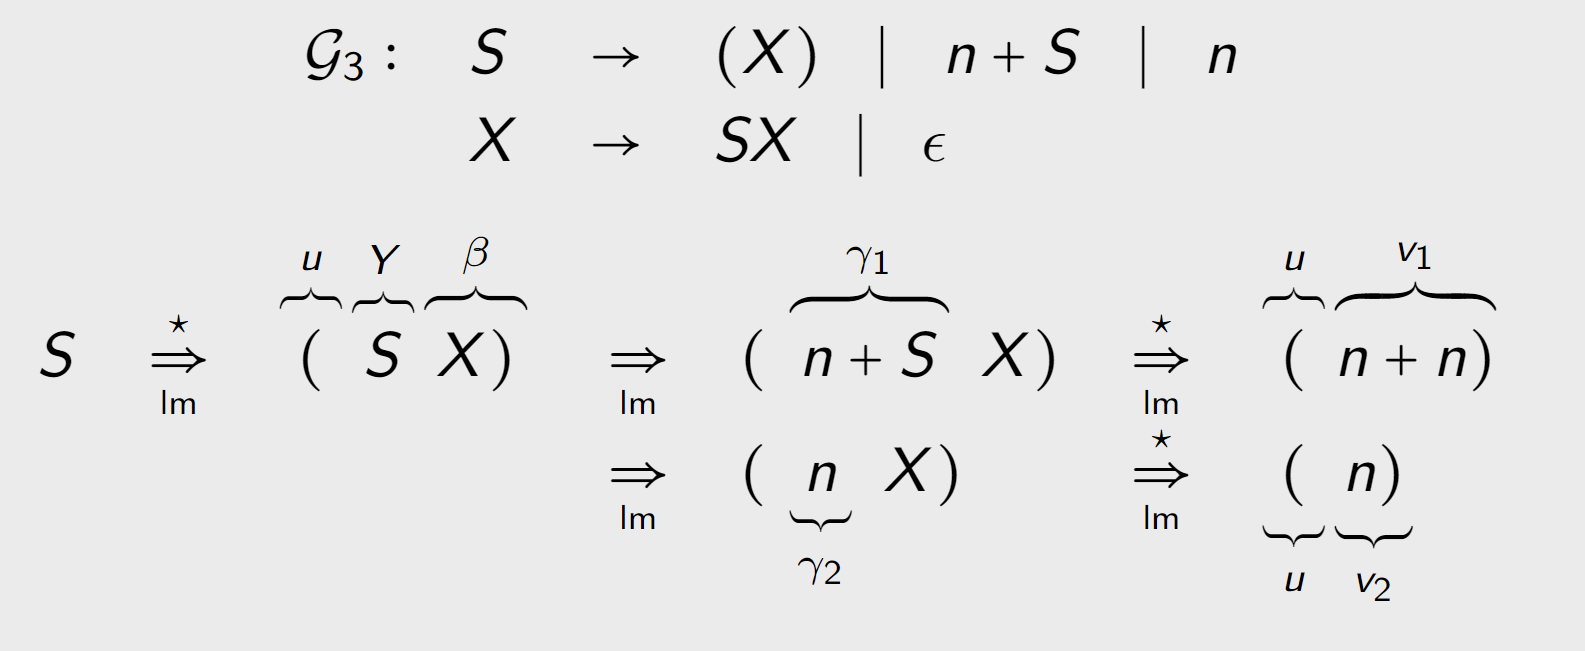
\includegraphics[scale=0.3]{img/cap5/ejemplo13.png}
        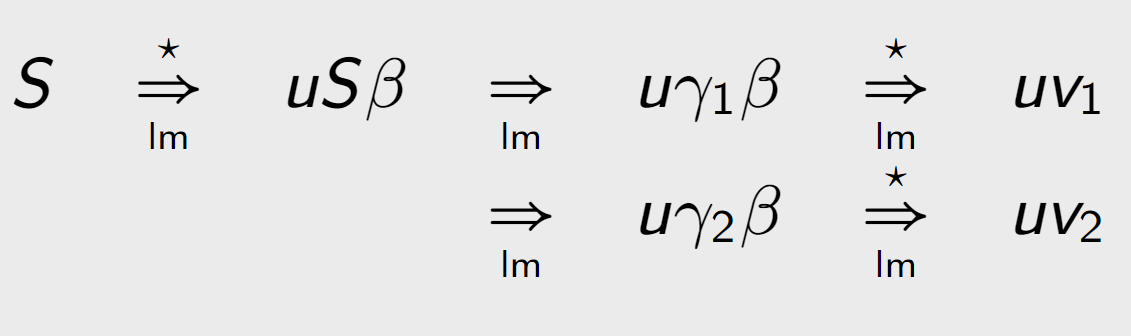
\includegraphics[scale=0.3]{img/cap5/ejemplo13_1.png}
    \end{figure}
    % \img{img/cap5/ejemplo13.png}{0.3}
    Como $v_1|_1 = v_2|_1 = n$ pero $\gamma_1 \neq \gamma_2$, entonces $\ca{G}_3$ NO es una gramática $\gll(1)$.
    % \img{img/cap5/ejemplo13_1.png}{0.3}
    \begin{itemize}
        \item Si $v_1|_2 = v_2|_2 = n+$, entonces $\gamma_1 = \gamma_2 = n + S$.
        \item Si $v_1|_1 = v_2|_1 = na$, con $a \neq +$, entonces $\gamma_1 = \gamma_2 = n$.
    \end{itemize}
    Por lo tanto, tenemos que $\gamma_1 = \gamma_2$ y entonces $\ca{G}_3$ es $\gll(2)$.
}
\ejemplo{Gramática NO $\gll(k)$}{}{
\img{img/cap5/ejemplo14.png}{0.35}
Como $v_1|_k = v_2|_k = (\overset{k}{\cdots}($ pero $\gamma_1 \neq \gamma_2$, entonces $\ca{G}_4$ NO es una gramática $\gll(k)$ para todo $k$.
    }

    \ejemplo{Gramática NO $\gll(k)$ transformada en $\gll(2)$}{}{
        La gramática $\ca{G}_4$ del ejemplo anterior se puede transformar para que sea $\gll(2)$ de la siguiente manera:
        \img{img/cap5/ejemplo15.png}{0.35}

        Queda como ejecicio para el lector demostrar que $\ca{G}_4'$ es $\gll(2)$.
    }

    \ejemplo{Lenguaje NO $\gll(k)$}{}{
        \img{img/cap5/ejemplo16.png}{0.35}
        Para todo $k\ge 1$, se tiene que $\ca{G}_5$ NO es una gramática $\gll(k)$. \medbreak

        Es posible demostrar que, para toda gramática $\ca{G}$ con $\ca{L}(\ca{G}_5) = \ca{L}(\ca{G})$, $\ca{G}$ NO es una gramática $\gll(k)$ para todo $k \geq 1$.
    }

    \subsubsection{Caracterización LL}
    Para esta parte es importante manejar las definiciones de prefijos vistas en la sección \ref{prefijos}. \medbreak

    Sea $\ca{G} = (V,\Sigma,P,S)$ una gramática libre de contexto \textbf{reducida} y $k \ge 1$. En base a esto definimos el siguiente teorema:

    \teorema{}{}{
        $\ca{G}$ es una gramática $\gll(k)$ si, y sólo si, para todas dos reglas distintas $Y\to\gamma_1,Y\to\gamma_2 \in P$ y para todo $S\ \overunder{\Rightarrow}{\mathrm{lm}}{*}\ uY\beta$, se tiene que:
        $$
            \first_k(\gamma_1 \beta)\ \cap\ \first_k(\gamma_2 \beta) = \varnothing
        $$

    }

    \paragraph{Demostración.} $(\Rightarrow)$ Por contrapositivo, supongamos que $v\in \first_k(\gamma_1 \beta) \cap \first_k(\gamma_2 \beta)$. Como $\ca{G}$ es reducida (sin variables inútiles), entonces
    \begin{align*}
        S \quad \overunder{\Rightarrow}{\mathrm{lm}}{*} \quad u Y \beta \quad & \overunder{\Rightarrow}{\mathrm{lm}}{}\ u \gamma_1 \beta \ \overunder{\Rightarrow}{\mathrm{lm}}{*} u v v_1 \\
                                                                              & \overunder{\Rightarrow}{\mathrm{lm}}{}\ u \gamma_2 \beta \ \overunder{\Rightarrow}{\mathrm{lm}}{*} u v v_2
    \end{align*}
    para algún $v_1,v_2 \in \Sigma^*$. Como $\gamma_1 \neq \gamma_2$, entonces $\ca{G}$ NO es $\gll(k)$. \medbreak

$(\Leftarrow)$ Por contrapositivo (de nuevo), supongamos que $\ca{G}$ no es $\gll(k)$. Como $\ca{G}$ no es $\gll(k)$, entonces tenemos derivaciones de la forma:
    \begin{align*}
        S \quad \overunder{\Rightarrow}{\mathrm{lm}}{*} \quad u Y \beta \quad & \overunder{\Rightarrow}{\mathrm{lm}}{}\ u \gamma_1 \beta \ \overunder{\Rightarrow}{\mathrm{lm}}{*} u v_1 \\
                                                                              & \overunder{\Rightarrow}{\mathrm{lm}}{}\ u \gamma_2 \beta \ \overunder{\Rightarrow}{\mathrm{lm}}{*} u v_2
    \end{align*}
    Vemos que $v_1|_k = v_2|_k = v$, pero $\gamma_1 \neq \gamma_2$. Por lo tanto, $v \in \first_k(\gamma_1 \beta) \cap \first_k(\gamma_2 \beta)$. \hfill $\blacksquare$ \bigbreak

    ¿Cómo usamos la caracterización del teorema para demostrar que una gramática es $\gll(k)$? Buscaremos condiciones más simples para verificar si una gramática es $\gll(k)$.

    \paragraph{Definición.} $\ca{G}$ es una gramática $\gll(k)$ \textbf{fuerte} si para todas dos reglas distintas $Y \to \gamma_1, Y\to \gamma_2 \in P$ se tiene que:
    \alignformula{
        \first_k(\gamma_1) \odot_k \follow_k(Y)\ \cap\ \first_k(\gamma_2) \odot_k \follow_k(Y) = \varnothing
    }

    \ejemplo{Si $\ca{G}$ es $\gll(k)$ fuerte, entonces $\ca{G}$ es $\gll(k)$}{}{
        Una gramática $\ca{G}$ que sea $\gll(k)$ fuerte siempre es $\gll(k)$, ya que si definimos dos conjuntos dados por el teorema de $\gll(k)$ $(F_1)$ y la definición de $\gll(k)$ fuerte $(F_2)$, dados por:
        \begin{align*}
            F_1 & = \first_k(\gamma_1 \beta)\ \cap \ \first_k(\gamma_2 \beta) = \first_k(\gamma_1) \odot_k \first_k(\beta) \ \cap \ \first_k(\gamma_2) \odot_k \first_k(\beta) \\
            F_2 & = \first_k(\gamma_1) \odot_k \first_k(Y) \ \cap \ \first_k(\gamma_2) \odot_k \first_k(Y) = \varnothing
        \end{align*}
        Entonces, tenemos que $F_1 \subseteq F_2$.
    }

    \ejemplo{Si $\ca{G}$ es $\gll(k)$, ¿es $\gll(k)$ fuerte?}{}{
        La respuesta directa es que no. Con un contrajemplo, tomemos la gramática $\ca{G}$ definida por
        \begin{align*}
            \ca{G}: \quad S & \to aXaa \mid bXba  \\
            X               & \to b \mid \epsilon
        \end{align*}
        \textbf{Recordatorio:} $\ca{G}$ es $\gll(k)$ si para todas dos reglas distintas $Y\to\gamma_1,Y\to\gamma_2 \in P$ y para todo $S \ \overunder{\Rightarrow}{\mathrm{lm}}{*}\ uY \beta$, se tiene que
        $$
            \first_k(\gamma_1 \beta) \ \cap \ \first_k(\gamma_2 \beta) = \varnothing
        $$
        \begin{itemize}
            \item Si $S \ \overunder{\Rightarrow}{\mathrm{lm}}{*}\ aXaa$, entonces $\first_2(baa) \ \cap \ \first_2(aa) = \varnothing$.
            \item Si $S \ \overunder{\Rightarrow}{\mathrm{lm}}{*}\ bXba$, entonces $\first_2(baa) \ \cap \ \first_2(ba) = \varnothing$
        \end{itemize}
        Por lo tanto, $\ca{G}$ es $\gll(2)$. \medbreak

        \textbf{Recordatorio:} $\ca{G}$ es una gramática $\gll(k)$ fuerte si para todas dos reglas distintas $Y\to\gamma_1,Y\to\gamma_2 \in P$ se tiene que:
        $$
            \first_k(\gamma_1) \odot_k \follow_k(Y)\ \cap\ \first_k(\gamma_2) \odot_k \follow_k(Y) = \varnothing
        $$
        Si vemos $X\to b$ y $X\to \epsilon$:
        \begin{align*}
            \first_2(b) & \odot_2 \follow_2(X)\ \cap\ \first_2(\epsilon) \odot_2 \follow_2(X)       \\
                        & = \{b\} \odot_2 \{aa, ba\} \ \cap \ \{\epsilon\} \odot_2 \{aa, ba\}       \\
                        & = \{ba, bb\} \ \cap \ \{aa, ba\}                                          \\
                        & = \{ba\} \qquad \qquad \text{y por ende $\ca{G}$ no es $\gll(2)$ fuerte.}
        \end{align*}
    }

    ¿Qué pasa con el caso $\gll(1)$? Supongamos que $\ca{G}$ es $\gll(1)$ y $Y\to\gamma_1, Y\to\gamma_2 \in P$ son reglas distintas.
    \begin{enumerate}
        \item Si $\epsilon \notin \first_1(\gamma_1)$ y $\epsilon \not\in \first_1(\gamma_2)$, entonces, por la caracterización de $\gll(1)$:
              \begin{align*}
                  \varnothing & = \first_1(\gamma_1 \beta) \ \cap \ \first_1(\gamma_2 \beta)                               \\
                              & = \first_1(\gamma_1) \ \cap \ \first_1(\gamma_2)                                           \\
                              & = \first_1(\gamma_1) \odot_1 \follow_1(Y) \ \cap \ \first_1(\gamma_2) \odot_1 \follow_1(Y)
              \end{align*}
        \item Si $\epsilon \in \first_1(\gamma_1)$ y $\epsilon \notin \first_1(\gamma_2)$, entonces, por la caracterización de $\gll(1)$:
              \begin{align*}
                  \varnothing & = \first_1(\gamma_1 \beta) \ \cap \ \first_1(\gamma_2 \beta)  \\
                              & = \first_1(\gamma_1 \beta) \ \cap \ \first_1(\gamma_2)        \\
                              & = \first_1(\gamma_1 \beta) \ \cap \ \first_1(\gamma_2 \beta') \\
              \end{align*}
              para todo $\beta' \in (V \cup \Sigma)^*$. Por lo tanto:
              \begin{align*}
                   & \first_1(\gamma_1) \odot_1 \follow_1(Y) \ \cap \ \first_1(\gamma_2) \odot_1 \follow_1(Y)                                                                                                            \\
                   & = \bigcup_{S \overunder{\Rightarrow}{\mathrm{lm}}{*}uY\beta} \first_1(\gamma_1 \beta) \ \cap \ \bigcup_{S \overunder{\Rightarrow}{\mathrm{lm}}{*}uY\beta'} \first_1 (\gamma_2 \beta') = \varnothing
              \end{align*}
    \end{enumerate}

    Por lo tanto, establecemos el siguiente teorema.

    \teorema{}{}{
        Una gramática $\ca{G}$ es $\gll(1)$ si, y sólo si, $\ca{G}$ es $\gll(1)$ \textbf{fuerte}, esto es, para todas dos reglas distintas $Y \to \gamma_1, Y \to \gamma_2 \in P$:
        $$
            \first_1(\gamma_1) \odot_1 \follow_1(Y)\ \cap\ \first_1(\gamma_2) \odot_1 \follow_1(Y) = \varnothing
        $$
    }
    La condición del teorema anterior se puede verificar en \textbf{tiempo polinomial} en $\ca{G}$.

    \subsection[Parsing con gramáticas LL(k)]{Parsing con gramáticas $\gll(k)$}
    \subsubsection{Algunas consideraciones}
    Considere la siguiente gramática $\ca{G}$:
    \begin{align*}
        S & \to Xa \mid Xb \\
        X & \to c
    \end{align*}

    ¿Es esta gramática del tipo $\gll(1)$? Podemos ver que $\first_1(\gamma_1 \beta) = \{c\}$ y $\first_1(\gamma_2 \beta) = \{c\}$, con $\gamma_1 = Xa$, $\gamma_2 = Xb$ y $\beta = \epsilon$. Por lo tanto su intersección no es vacía y entonces $\ca{G}$ no es $\gll(1)$. ¿Podemos establecer una solución para este problema?

\paragraph{Factorización.} En general, si tenemos una regla:
$$
    X \to \gamma\alpha_1 \mid \gamma \alpha_2
$$
siempre podemos ``\textbf{factorizar}'' la regla manteniendo la semántica, como:
\begin{align*}
    X  & \to \gamma X'              \\
    X' & \to \alpha_1 \mid \alpha_2
\end{align*}

Considere ahora la siguiente gramática $\ca{G}$:
$$
    E \to E * E \mid n
$$

¿Es esta gramática del tipo $\gll(1)$? ¿$\gll(k)$? Pues no es ninguna. El problema con esta gramática es su recursividad, en específico, por la izquierda.

\paragraph{Definición.} Una gramática $\ca{G}$ se dice \textbf{recursiva por la izquirrda} si existe $X \in V$ tal que:
\alignformula{
    X \overunder{\Rightarrow}{}{+} X\gamma \quad \text{para algún }\gamma \in (V \cup \Sigma)^*
}

\teorema{}{}{
    Si $\ca{G}=(V,\Sigma,P,S)$ es una gramática reducida y recursiva por la izquierda, entonces $\ca{G}$ NO es $\gll(k)$ para todo $k \ge 1$.
}
\paragraph{Demostración.} Por simplicidad, suponga que $X \to X\beta \in P$ y $X \to w \in P$. \medbreak

Como $\ca{G}$ es reducida, entonces existe una derivación $S \overunder{\Rightarrow}{\mathrm{lm}}{*} uX\gamma$:
$$
    S \ \overunder{\Rightarrow}{\mathrm{lm}}{*} \ uX\gamma \ \overunder{\Rightarrow}{\mathrm{lm}}{} \ \overset{n\text{-veces}}{\cdots}\ \overunder{\Rightarrow}{\mathrm{lm}}{} \ uX \beta^n\gamma
$$
Por \textbf{contradicción}, suponga que $\ca{G}$ es $\gll(k)$. Por lo tanto:
$$
    \first_k(X\beta^{n+1}\gamma) \ \cap \ \first_k(w \beta^n \gamma) = \varnothing
$$
Suponga que $\beta \overunder{\Rightarrow}{}{*} v \in \Sigma^*$ y $\gamma \overunder{\Rightarrow}{}{*} v' \in \Sigma^*$. Con $n = k$, tendremos que
$$
    (wv^k v')|_k \quad \in \quad \first_k(X\beta^{k+1}\gamma) \ \cap \ \first_k(w \beta^k\gamma) \quad \rightarrow\leftarrow \text{ (¡contradicción! el conjunto no es vacío)}
$$
\hfill $\blacksquare$ \bigbreak

Hablemos de recursión \textbf{inmediata} por la izquierda. Suponga que existe $X \in V$ tal que:
$$
    X \to X \alpha_1 \mid \cdots \mid X \alpha_m \mid \beta_1 \mid \cdots \mid \beta_n
$$
¿Cómo podemos \textbf{eliminar} la recursión inmediata por la izquierda? Consideramos la misma gramática pero \textbf{cambiando} las reglas de $X$ por:
\begin{align*}
    X  & \to \beta_1 X' \mid \cdots \mid \beta_n X'                 \\
    X' & \to \alpha_1 X' \mid \cdots \mid \alpha_m X' \mid \epsilon
\end{align*}
\ejemplo{Eliminando recursión inmediata}{}{
    \img{img/cap5/ejemplo19.png}{0.4}
}

\teorema{}{}{
    Sea $\ca{G}$ una gramática tal que existe $X \in V$:
    $$
        X \to X \alpha_1 \mid \cdots \mid X \alpha_m \mid \beta_1 \mid \cdots \mid \beta_n
    $$
    Sea $\ca{G}'$ la misma gramática $\ca{G}$ pero cambiando las reglas de $X$ por:
    \begin{align*}
        X  & \to \beta_1 X' \mid \cdots \mid \beta_n X'                 \\
        X' & \to \alpha_1 X' \mid \cdots \mid \alpha_m X' \mid \epsilon
    \end{align*}
    Entonces $\ca{L}(\ca{G})=\ca{L}(\ca{G}')$
}

\paragraph{Demostración.} Una derivación por la izquierda de $X$ en $\ca{G}$:
$$
    X \ \underset{\mathrm{lm}}{\Rightarrow} \ X \alpha_{i_1} \ \underset{\mathrm{lm}}{\Rightarrow} \ X \alpha_{i_2} \alpha_{i_1} \ \underset{\mathrm{lm}}{\Rightarrow} \ \cdots \ \underset{\mathrm{lm}}{\Rightarrow}\ X \alpha_{i_p} \alpha_{i_{p-1}} \cdots \alpha_{i_1} \ \underset{\mathrm{lm}}{\Rightarrow} \ \beta_j \alpha_{i_p} \alpha_{i_{p-1}} \cdots \alpha_{i_1}
$$
Una derivación por la derecha de $X$ en $\ca{G}'$ \textbf{equivalente}:
$$
    X \ \underset{\mathrm{rm}}{\Rightarrow} \ \beta_j X' \ \underset{\mathrm{rm}}{\Rightarrow} \ \beta_j \alpha_{i_p} X' \ \underset{\mathrm{rm}}{\Rightarrow} \ \cdots \ \underset{\mathrm{rm}}{\Rightarrow}\ \beta_j \alpha_{i_p} \cdots \alpha_{i_2} \alpha_{i_1} X' \ \underset{\mathrm{rm}}{\Rightarrow} \ \beta_j \alpha_{i_p} \alpha_{i_{p-1}} \cdots \alpha_{i_1}
$$
\hfill $\blacksquare$ \bigbreak

Ahora, ¿qué pasa si la recursión por la izquierda es \textbf{no-inmediata}? Considere la siguiente gramática \textbf{recursiva por la izquierda}:
\begin{align*}
    S & \to Xa \mid b \\
    X & \to Yc        \\
    Y & \to Xd \mid e
\end{align*}

¿Cómo eliminamos la recursión por la izquierda no-inmediata?
\paragraph{Estrategia.} Dado $V = \{X_1,\ldots,X_n\}$, removemos la recursión inductivamente en $n$, tal que, en cada paso $i$ de la inducción, se cumplira que para todo $i,j\leq n$:
$$
    \text{si } X_i \to X_j \alpha, \text{ entonces } i < j
$$

\vspace{-15pt}
\begin{algorithm}[hbt!]
    % \caption*{An algorithm with caption}\label{alg:two}
    \setstretch{1.25}
    \DontPrintSemicolon
    \SetKwFunction{FEliminarRecursion}{EliminarRecursion}
    \SetKwProg{Fn}{Function}{:}{}
    \SetKwInOut{Input}{input}\SetKwInOut{Output}{output}
    \Input{Gramática $\ca{G}=(V,\Sigma,P,S)$ y $V=\{X_1,\ldots,X_n\}$}
    \Output{Gramática $\ca{G}$ sin recursión por la izquierda}
    \Fn{\FEliminarRecursion{$\ca{G}$}}{
        $P':=P$

        \For{$i=1$ \KwTo $n$}{
            \For{$j=1$ \KwTo $i-1$}{
                \ForEach{$X_i \to X_j \gamma \in P'$}{
                    \ForEach{$X_j \to \alpha \in P'$}{
                        $P' := P' \cup \{X_i \to \alpha\gamma\}$
                    }
                    $P' := P' - \{X_i \to X_j \gamma\}$
                }
            }
            Remover recursión inmediata para $X_i$ en $P'$ (si existe)
        }
        $V' := \{X_1,\ldots,X_n\} \cup \{X_1',\ldots,X_n'\}$

        \Return{$(V',\Sigma,P',S)$}
    }
\end{algorithm}

Queda como ejercicio propuesto al lector demostrar la correctitud del algoritmo.

\ejemplo{Eliminando recursión}{}{
    \begin{align*}
        E & \to E + T \mid T \\
        T & \to T * F \mid F \\
        F & \to (E) \mid n
    \end{align*}
    Eliminando la \textbf{recursión inmediata} de $E$:
    \begin{align*}
        E  & \to TE'                \\
        E' & \to +TE' \mid \epsilon \\
        T  & \to T * F \mid F       \\
        F  & \to (E) \mid n
    \end{align*}
    Eliminando la \textbf{recusión inmediata} de $T$:
    \begin{align*}
        E  & \to TE'                \\
        E' & \to +TE' \mid \epsilon \\
        T  & \to FT'                \\
        T' & \to *FT' \mid \epsilon \\
        F  & \to (E) \mid n
    \end{align*}
}
\vspace{-10pt}
\paragraph{Conclusión.} Es \textbf{posible eliminar} la recursividad por la izquierda, pero esto \textbf{NO asegura} que el resultado sea una gramática $\gll(k)$ para algún $k$.

\subsubsection[Parsing de LL(k)]{Parsing de $\gll(k)$}
\fig{img/cap5/parsing_llk.png}{0.4}{Máquina de parsing}

\paragraph{Definición.} Sea $\Sigma$ un alfabeto finito. Se definen los siguientes conjuntos de palabras:
\begin{itemize}
    \item $\dot{\Sigma}= \Sigma^* \times \Sigma^*$
    \item $\dot{\Sigma}^{\le k} = \{ (u,v) \in \dot{\Sigma} \mid |uv| \le k \}$
    \item $\dot{\Sigma}_{\#}^{\le k} = \{ (u,v) \in \dot{\Sigma} \mid |uv| \le k \} \cup \{ (u,v\#) \mid (u,v) \in \dot{\Sigma} \mid |uv| < k \}$
\end{itemize}

\paragraph{Notación.} En vez de usar $(u,v) \in \dot{\Sigma}_{\#}^{\le k}$, escribiremos $u.v \in \dot{\Sigma}_{\#}^{\le k}$. El par $\epsilon.\epsilon$ lo denotaremos solamente por $\epsilon$.

\paragraph{Definición.} Un transductor apilador con $k$-lookahead ($k$-PDT) es una tupla:
\alignformula{
    \ca{T} = (Q, \Sigma, \Omega, \Delta, q_0, F)
}

\begin{itemize}
    \item $Q$ es un conjunto finito de estados.
    \item $\Sigma$ es el alfabeto de input.
    \item $\Omega$ es el alfabeto de output.
    \item $\Delta \subseteq Q^{+} \times \dot{\Sigma}_{\#}^{\leq k} \times(\Omega \cup\{\epsilon\}) \times Q^*$ es la relación de transición.
    \item $q_0 \in Q$ es un conjunto de estados iniciales.
    \item $F \subseteq Q$ es el conjunto de estados finales.
\end{itemize}

\paragraph{Definición.} Una \textbf{configuración} de $\ca{T}$ es una tupla:
\alignformula{
    \left(q_1 \ldots q_k, w, o\right) \in\left(Q^{+}, \Sigma^* \cdot\{\#\}, \Omega^*\right)
}
\begin{itemize}
    \item $q_1\ldots q_k$ es el contenido del stack con $q_1$ el tope del stack.
    \item $w$ es el contenido del input.
    \item $o$ es el contenido del output.
\end{itemize}
Decimos que una configuración:
\begin{itemize}
    \item $(q_0, w\#, \epsilon)$ es \textbf{inicial} y
    \item $(q_f, \#, o)$ es \textbf{final} si $q_f \in F$.
\end{itemize}

\paragraph{Definición.} Se define la relación $\vdash_{\ca{T}}$ de \textbf{siguiente-paso} entre configuraciones de $\ca{T}$:
\alignformula{
    \left(\gamma_1, w_1, o_1\right)\ \vdash_\mathcal{T}\ \left(\gamma_2, w_2, o_2\right)
}
si, y sólo si, existe $(\alpha,u.v,a,\beta) \in \Delta$, $\gamma \in \Gamma^*$ y $w \in \Sigma^* \cdot \{\#\}$ tal que:
\begin{itemize}
    \item \textbf{Stack:} $\gamma_1 = \alpha \cdot \gamma$ y $\gamma_2 = \beta \cdot \gamma$
    \item \textbf{Look-ahead:} $w_1 = u \cdot v \cdot w$ y $w_2 = v \cdot w$
    \item \textbf{Output:} $o_2 = o_1 \cdot a$
\end{itemize}
Se define $\vdash_{\ca{T}}^*$ como la clausura \textbf{refleja} y \textbf{transitiva} de $\vdash_{\ca{T}}$.

\paragraph{Definición.} $\ca{T}$ \textbf{entrega} $o$ con \textbf{input} $w$ si existe una configuración inicial $(q_0, w\cdot \#, \epsilon)$ y una configuración final $(q_f, \#, o)$ tal que:
$$
    \left(q_0, w \cdot \#, \epsilon\right) \vdash_{\mathcal{T}}^*\left(q_f, \#, o\right)
$$
Se define la función $\llbracket \ca{T} \rrbracket: \Sigma^* \to 2^{\Omega^*}$:
\alignformula{
    \llbracket \mathcal{T} \rrbracket(w)=\left\{o \in \Omega^* \mid \mathcal{T} \text { entrega } o \text { con input } w\right\}
}

\paragraph{Definición.} $\ca{T}$ es \textbf{determinista} si para todo $\left(\alpha_1, u_1.v_1, a_1, \beta_1\right),\left(\alpha_2, u_2.v_2, a_2, \beta_2\right) \in \Delta$ con \\
$\left(\alpha_1, u_1.v_1, a_1, \beta_1\right) \neq\left(\alpha_2, u_2.v_2, a_2, \beta_2\right)$ se cumple que
\alignformula{
    \alpha_1 \text { NO es prefijo de } \alpha_2 \quad \text{o} \quad u_1 v_1 \text { NO es prefijo de } u_2 v_2 \text {. }
}
\textit{``Para cualquier configuración $(\gamma, w, o)$ existe \textbf{a lo más} una configuración $(\gamma', w', o)$ tal que $(\gamma,w,o) \vdash_{\ca{T}}^* (\gamma',w', o')$''} \medbreak

La \textbf{ventaja} de un $k$-PDT determinista es que nos aseguramos de que siempre obtenemos un solo output para cada input (el no-determinismo nos podría generar muchos outputs distintos).

\paragraph{Construcción del parser.} Sea $\ca{G}=(V,\Sigma, P, S)$ una gramática $\gll(k)$ fuerte. Se define el $k$-PDT para $\ca{G}$:
\alignformula{
    \ca{T}[\ca{G}]= \Big( V\cup \Sigma \cup \{q_0,q_f\},\Sigma, \underbrace{P}_\Omega, \Delta, q_0, \{q_f\} \Big)
}
La relación de transición $\Delta$ de define como:
\begin{table}[H]
    \centering
    \begin{tabular}{rl}
        \textbf{Inicio:}   & $(q_0, \epsilon., \epsilon, S\cdot q_f)$                                                \\
        \textbf{Reducir:}  & $(a, a., \epsilon, \epsilon)$ para cada $a \in \Sigma$                                  \\
        \textbf{Expandir:} & $(X, .u, p, \gamma)$                                                                    \\
                           & para cada $p:=(X\to\gamma) \in P$ tal que $u \in \first_k(\gamma) \odot_k \follow_k(X)$
    \end{tabular}
\end{table}

\paragraph{Propiedades.} $\ca{T}[\ca{G}]$ tiene las siguientes propiedades:
\begin{enumerate}
    \item $\ca{T}[\ca{G}]$ es un $k$-PDT \textbf{determinista} si, y sólo si, $\ca{G}$ es $\gll{k}$ fuerte.
    \item Si $w \notin \ca{L}(\ca{G})$ entonces $\llbracket \ca{T} \rrbracket (w) = \varnothing$.
    \item Si $w \in \ca{L}(\ca{G})$ entonces $\llbracket \ca{T} \rrbracket(w) = \{r_1 \ldots r_m\}$ es una derivación por la izquierda de $\ca{G}$ sobre $w$.
\end{enumerate}

\paragraph{Algoritmo.} Para una gramática $\gll(k)$ $\ca{G}$ y una palabra $w \in \Sigma^*$:
\begin{enumerate}
    \item Construya el $k$-PDT determinista $\ca{T}[\ca{G}]$ a partir de $\ca{G}$.
    \item Ejecute $\ca{T}[\ca[G]]$ sobre $w$.
\end{enumerate}

Como $\ca{T}[\ca{G}]$ es determinista, entonces el algoritmo toma \textbf{tiempo lineal} en $w$.

\paragraph{Tabla predictiva para $\gll(k)$ fuerte.} Sea $\ca{G}=(V,\Sigma, P, S)$ una gramática $\gll(k)$ fuerte. Para cada $u \in \Sigma^k \cup \Sigma^{<k}\cdot \{\#\}$, se define $M[X,u] \in (V\cup \Sigma)^* \cup \{\texttt{ERROR}\}$:

\alignformula{
    M[X, u]= \begin{cases}
        \quad\gamma       & \text { si } X \rightarrow \gamma \in P \text { y } u \in \first_k(\gamma) \odot_k \follow_k(X) \\
        \texttt { ERROR } & \text { en otro caso. }
    \end{cases}
}
El computo de la tabla predictiva puede tomar \textbf{tiempo exponencial} en $|\ca{G}|$ y $k$.

\paragraph{Caso especial: tabla predictiva para $\gll(1)$.} Sea $\ca{G}=(V,\Sigma, P, S)$ una gramática $\gll(1)$ fuerte. Para cada $a \in \Sigma \cup \{\#\}$, se define $M[x,a] \in (V \cup \Sigma)^* \cup \{\texttt{ERROR}\}$:
\alignformula{
    M[X, a]= \begin{cases}
        \quad \gamma    & \text { si } X \rightarrow \gamma \in P \text { y } a \in \first_1(\gamma)                            \\
        \quad \gamma    & \text { si } X \rightarrow \gamma \in P, \epsilon \in \first_1(\gamma) \text { y } a \in \follow_1(X) \\
        \text { ERROR } & \text { en otro caso. }
    \end{cases}
}
Este cálculo se puede hacer en tiempo $\ca{O}(|V|\cdot|P|)$.

\ejemplo{Tabla predictiva}{}{
    \img{img/cap5/ejemplo21.png}{0.5}
}
